\documentclass[border=10pt]{standalone}
\usepackage{tikz}
\usetikzlibrary{calc}

\tikzstyle{vertex}=[circle,draw,fill=black!20,minimum size=0.3cm,inner sep=0pt]
\tikzstyle{selected vertex} = [vertex, fill=red!24]
\tikzstyle{edge} = [draw,thick,-]
\tikzstyle{weight} = [font=\small]
\tikzstyle{selected edge} = [draw,line width=3pt,-,red!70]
\tikzstyle{ignored edge} = [draw,line width=5pt,-,black!20]

\begin{document}
\noindent
    \centering
    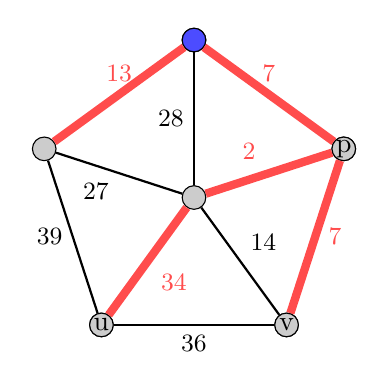
\begin{tikzpicture}[scale=1.0,transform shape,auto,swap]
        \foreach \i in {0,1,...,4}{
            \node[vertex] (v\i) at ({2*sin(\i*72)}, {2*cos(\i*72)}) {};
        }
        \node[vertex] (v5) at (0, 0) {};
        \node[vertex,fill=blue!70] (v0_text) at (v0) {};
        \node[vertex] (v1_text) at (v1) {p};
        \node[vertex] (v2_text) at (v2) {v};
        \node[vertex] (v3_text) at (v3) {u};

        \path[edge] (v0) -- node[weight] {28} (v5);
        \path[selected edge] (v1) -- node[weight] {2} (v5);
        \path[edge] (v2) -- node[weight] {14} (v5);
        \path[selected edge] (v3) -- node[weight] {34} (v5);
        \path[edge] (v4) -- node[weight] {27} (v5);
        \path[selected edge] (v0) -- node[weight,above] {7} (v1);
        \path[selected edge] (v1) -- node[weight,right] {7} (v2);
        \path[edge] (v2) -- node[weight,below] {36} (v3);
        \path[edge] (v3) -- node[weight,left] {39} (v4);
        \path[selected edge] (v4) -- node[weight,above] {13} (v0);
    \end{tikzpicture}
\end{document}
